\documentclass[a4paper]{scrartcl}
\usepackage[utf8]{inputenc}
\usepackage[english]{babel}
\usepackage{graphicx}
\usepackage{lastpage}
\usepackage{pgf}
\usepackage{wrapfig}
\usepackage{fancyvrb}
\usepackage{fancyhdr}
\usepackage{listings}
\pagestyle{fancy}
\usepackage{libertine}
\renewcommand*\familydefault{\sfdefault}  %% Only if the base font of the document is to be sans serif
\usepackage[T1]{fontenc}
\usepackage{courier}
\usepackage[parfill]{parskip}

\graphicspath{ {./images/} }

% Create header and footer
\headheight 27pt
\pagestyle{fancyplain}
\lhead{\footnotesize{Internet Applications, ID1354}}
\chead{\footnotesize{Assignment 1: HTML \& CSS}}
\rhead{}
\lfoot{}
\cfoot{\thepage\ (\pageref{LastPage})}
\rfoot{}

% Create title page
\title{Assignment 1: HTML \& CSS}
\subtitle{Internet Applications, ID1354}
\author{Emil Tullstedt [emiltu@kth.se]}
\date{2014-09-02}

\lstset{
	basicstyle=\footnotesize\ttfamily, 
	numbers=left,
	breaklines=true,
	frame=l,
	keywordstyle=\bfseries\color{blue!40!black},
    stringstyle=\color{red},
    commentstyle=\color{green},
    identifierstyle=\color{black},
    showstringspaces=false
}

\begin{document}

\maketitle

\section{Introduction}

The first assignment in ID1354 is to create a recipe website using HTML and CSS. This report describes the process and result of one such solution made by Emil Tullstedt.

The requirements for the website is to contain two recipes, one index page welcoming the users and a calendar page where the site have a "meal of the day" for a month. The website shall also be valid and work in common and modern browsers (IE10+, Fx26+ and corresponding Safari and Chrome versions).

\section{Method}

\subsection{HTML}

HTML is the single uniting factor of every website. A well programmed text based informational website has clear HTML which can be understood both when rendered \textit{as-is} without accompanying JavaScript or CSS and also by someone who has a basic level of understanding by looking at the HTML in text format.

This level of clarity was achieved in this project by making sure to add the HTML structure first and afterward making sure it looks nice and works well by adding JavaScript and CSS behavior, using the \texttt{h1-h6} for different title layers, the new HTML5 section tags and generally naming stuff understandably.

\subsection{CSS}

The standardized way of telling browsers how websites are layouted is called CSS, or Cascading Style Sheets. CSS works by looking for the most specific definition of style available, and with the "new" CSS3 \textit{media queries}, the site can be reflowed depending on what is being used for viewing the website. The project relies heavily on the different width features of these media queries to offer a sensible viewing experience on any commonly found screen size.

\subsection{Fonts}
\label{subsec:Fonts}

When developing a web site, one of the key elements to think about is which fonts are used. Trusting the default font to be a sane default is quite often problematic since font qualities generally differ greatly between different browsers. When using unicode emoticons for example, Twitter replaces them with images to stop the issue where different users sees different emoticons. This can, in the case of Twitter, mean the difference between people understanding each other and not. As thus, you may understand the importance of deciding for a font.

How many fonts that are used in a website is a combination of aesthetics and page weight (see section \ref{subsec:PageWeight}). Simply put, a stylized font for titles and readable font for the text is probably the best choice.

When having decided for a font, it is important to offer the font in different font-formats to the end user. This can either be achieved by using one of many font delivery networks out there or if you wish to serve the font from your own server by using a conversion tool, e.g. FontSquirrel's webfont generator\footnote{http://www.fontsquirrel.com/tools/webfont-generator}.

\subsection{Validation}

When developing for the web, making sure the website works in all different kinds of browsers is important as the purpose of the web is to have a single point of reference which is freely accessible for everyone. Following the standards isn't hard when you use the proper tools to ensure compliance with different browsers. A sample set of tools that are used to ensure compliance in this project are:

\begin{enumerate}
\item The W3C HTML validator\footnote{http://validator.w3.org} and it's accompanying CSS validator
\item The Can I Use website\footnote{http://caniuse.com/} lists which features are compatible with which browser
\item The HTML5 specifications\footnote{http://www.w3.org/TR/html5/}
\item The CSS3 media queries specification\footnote{http://www.w3.org/TR/css3-mediaqueries/}
\item Microsoft's website screenshot tool\footnote{https://modern.ie/en-gb/screenshots} to quickly get images of the websites in different browsers
\end{enumerate}

By intelligently using these tools and resources often and throughout the development time can be shortened as the need for time-consuming browser-specific fixes can be cut.

\subsection{Page Weight}
\label{subsec:PageWeight}

One easily dismissed practice when developing for the web is caring for the users' resources. The big problem is when developers don't care for the limited amount of resources available to a user.

Limited resources is an increasingly large issue with a heavy increase of ISPs that impose some kind of rate limiting on their users, even at low levels of data transfer in the numbers of .5-5 GB/month of data in 4G data rates. Even 5 GB is just a few minutes of downloading at full speed.

\section{Result}
\label{sec:results}

The fonts that were chosen to use for the project site is Lobster and Lato according to the suggestions from subsection \ref{subsec:Fonts} where Lobster was used as a title font and Lato was used for the body. The fonts used can be seen in figure \ref{fig:fonts}.

\begin{figure}[h]
  \begin{center}
    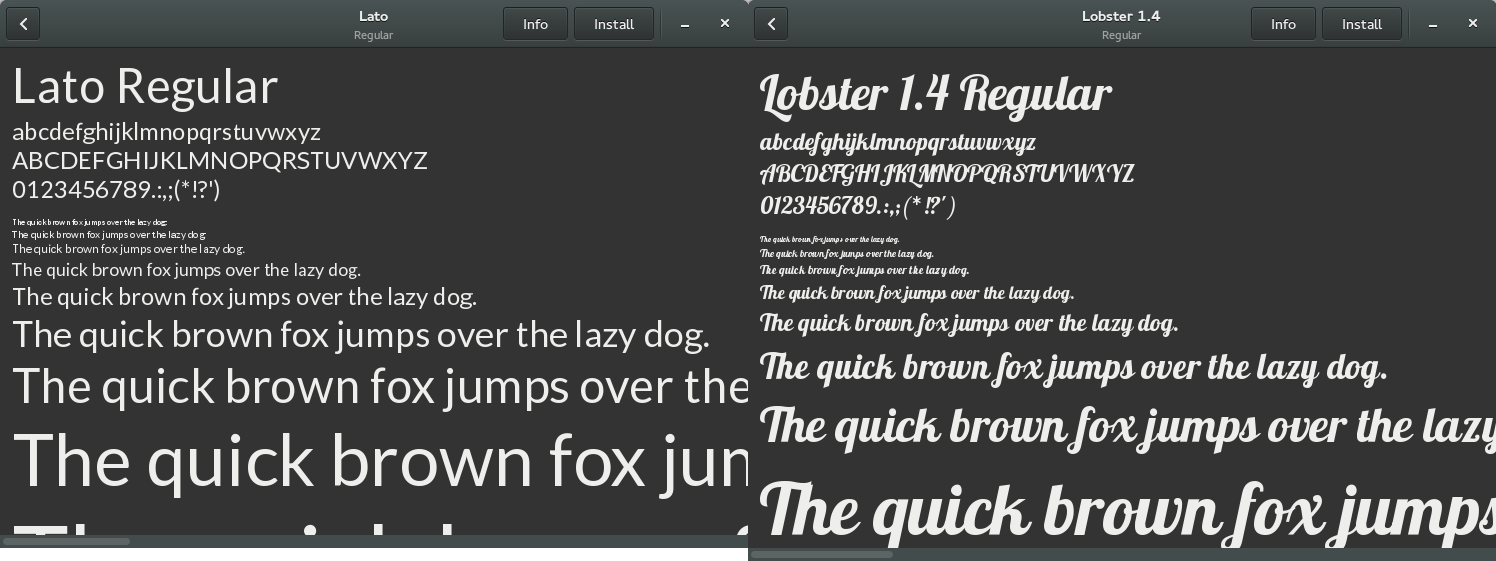
\includegraphics[scale=0.3]{fonts.png}
    \caption{The fonts used for the website}
    \label{fig:fonts}
  \end{center}
\end{figure}

For the site to feel snappy the images that are being loaded on the different pages needs to be sized correctly already on the server. By using the \texttt{ImageMagick} toolkit to re-size the images to a couple of different resolutions twenty-fold savings in terms of file size could be made, as shown in table \ref{tab:ressize}. Because the HTML-\texttt{picture} element isn't implemented everywhere yet, JavaScript is still needed in order to actually load larger images for bigger viewports. Thus the larger scale images weren't put to use anywhere in this version of the website.

% The following lines show how to create a table.
 \begin{table}[h]
   \centering
   \begin{tabular}{|l|r|r|}
     \hline
     File & Resolution & Size\\
     \hline
     meatballs.jpg & 2048x1536 & 1.606MB\\
     \hline
     meatballs720.jpg & 720x540 & 309KB\\
	 \hline
	 meatballs480.jpg & 480x360 & 172KB\\   
     \hline
     meatballs320.jpg & 320x240 & 103KB\\
     \hline
     meatballs128.jpg & 128x96 & 51.8KB\\
     \hline
   \end{tabular}
   \caption{Resolution-Size relationship}
   \label{tab:ressize}
 \end{table}

When the website was developed, the first thing to do was a super simple front page. This was achieved by first creating a HTML structure which contained the necessary HTML-wrappings and then adding CSS. By doing so, early versions of the site can be seen in figure \ref{fig:frontpage no css}.

\begin{figure}[!h]
  \begin{center}
    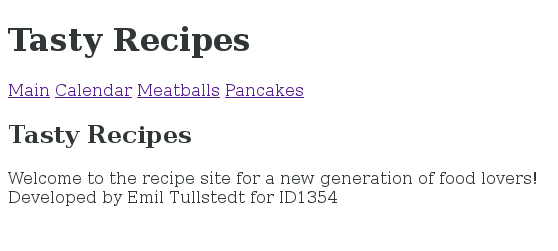
\includegraphics[scale=0.6]{frontpageWOcss.png}
    \caption{Early versions of the frontpage looks without any CSS}
    \label{fig:frontpage no css}
  \end{center}
\end{figure}

\begin{figure}[!h]
  \begin{center}
    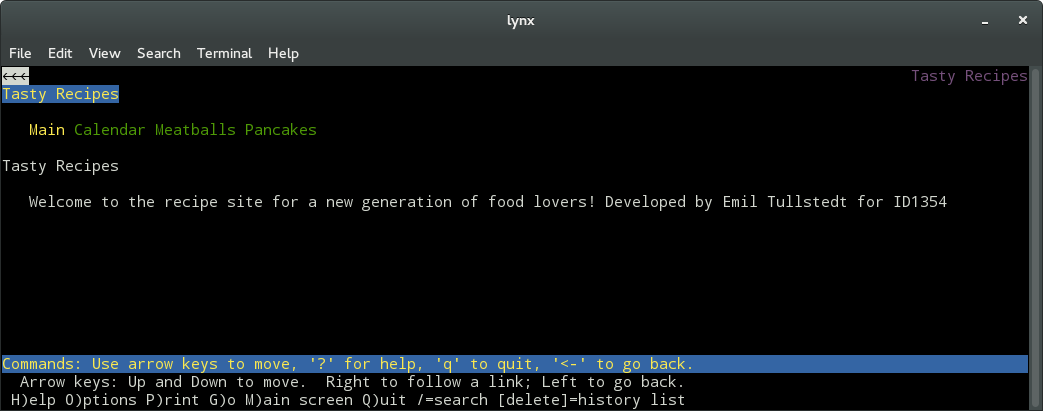
\includegraphics[scale=0.4]{lynx.png}
    \caption{The early version of the frontpage in a text based web browser (Lynx)}
    \label{fig:lynx}
  \end{center}
\end{figure}

\begin{figure}[!h]
  \begin{center}
    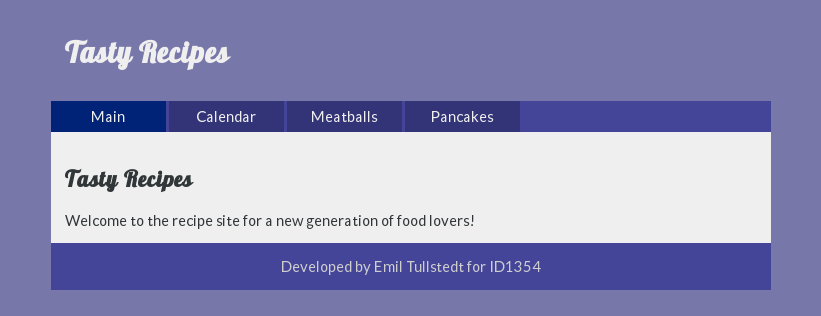
\includegraphics[scale=0.4]{frontpage1.png}
    \caption{The early version of the frontpage with CSS}
    \label{fig:early frontpage}
  \end{center}
\end{figure}

Another advantage by doing a clean structure is that it works even in text based web browser, as demonstrated in figure \ref{fig:lynx}. After this, the structure was stylized using CSS, resulting in figure \ref{fig:early frontpage}. Using CSS with media queries, the website could easily adapt for four different dimensions 

\begin{enumerate}
\item \textit{low resolution} mostly vertical mode (for screen-sizes 320-480px in width)
\item \textit{mediumlow resolution} for tablets and landscape phones (sizes between 480-720px), which has a few horizontal properties, but otherwise is mostly like the low resolution mode.
\item \textit{standard resolution} for screen-sizes 720 up to 1200px in width, which is the standard look of the website with lots of horizontal features
\item \textit{high resolution} for screen-sizes above 1200px in width. This adds a few horizontal features to the standard resolution and makes the entire site wider. Higher width resolutions would get readability issues if this resolution were to be any wider, especially as there currently isn't any need for further use of the horizontal space.
\end{enumerate}

\begin{figure}[!h]
  \begin{center}
    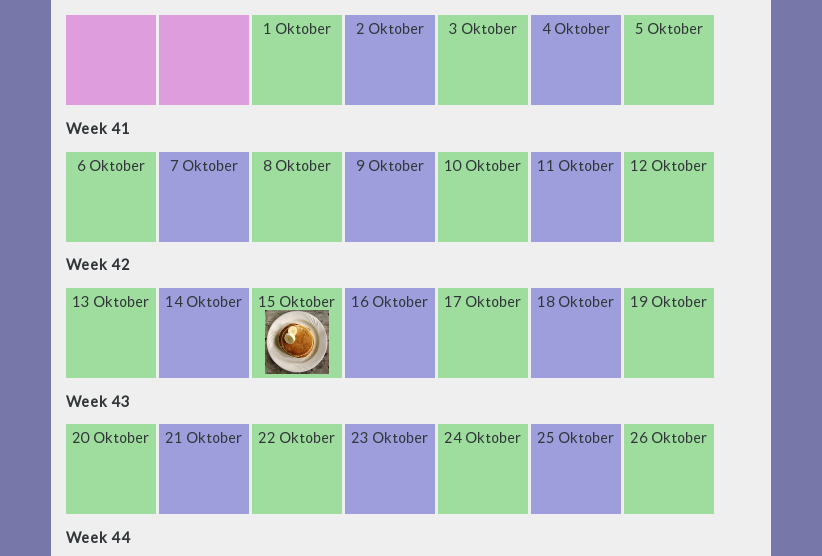
\includegraphics[scale=0.4]{calendargrid.png}
    \caption{The "standard" version of the calendar}
    \label{fig:calgrid}
  \end{center}
\end{figure}

\begin{figure}[!h]
  \begin{center}
    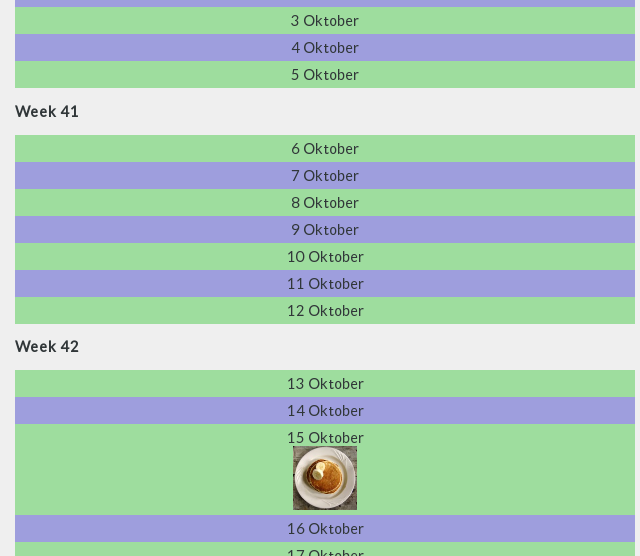
\includegraphics[scale=0.4]{calendarvert.png}
    \caption{The mobile and low-resolution screen version of the calendar}
    \label{fig:calvert}
  \end{center}
\end{figure}

When continuing with the development of the \texttt{calendar.html} page, the purpose was to make a grid-style one-month calendar, which typically can be achieved using tables in HTML. After some thought, using a \texttt{div}-based calendar scheme would simplify the accessibility and responsiveness customization process later on.

The calendar is shown in the original grid layout style for the standard and above resolutions (see figure \ref{fig:calgrid}), but is rescaled into a vertical calendar look for smaller screens to make sure every item gets enough space to be clickable if there's a link to a recipe on the date (see figure \ref{fig:calvert}).

The small screen calendar mode also collapses the empty dates so that they do not take up unnecessary space and forces the user to scroll excessively.

The calendar's variable grid look is made up using the CSS selectors \texttt{:nth-type-of} which is fully supported in all modern browsers\footnote{See http://www.w3.org/TR/css3-selectors/}. CSS selectors is a good alternative to JavaScript for coloring certain child elements without breaking encapsulation and starting to tweak style in HTML or using multiple classes.

For the "empty" dates (i.e. offset days in the calendar, either at the beginning or end of the month\footnote{Unless you're changing calendar system from Julian to Gregorian or vice verse. In that case, you'll probably need a few "empty" days in the middle of the month}) another class \texttt{empty} was used to extinguish these days from existing dates and enabling them to be removed in the low resolution versions.

%images for recipes
\begin{figure}[!h]
  \begin{center}
    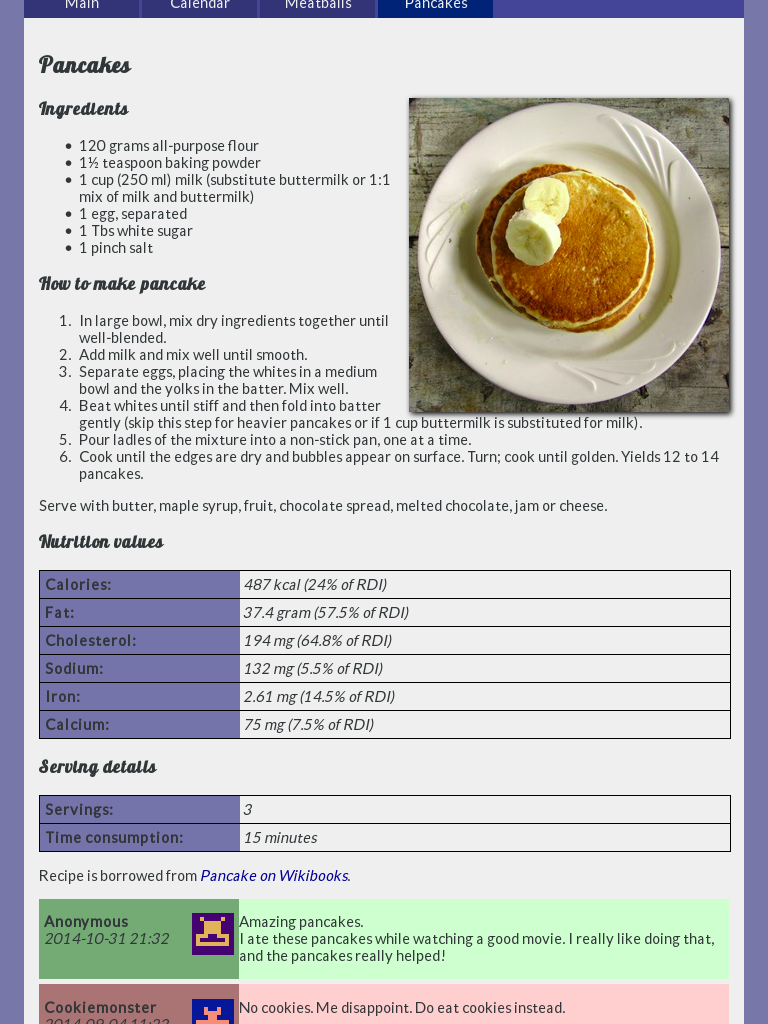
\includegraphics[scale=0.4]{pancakestd1.png}
    \caption{Recipe overview in standard resolution}
    \label{fig:pancakestd}
  \end{center}
\end{figure}

\begin{figure}[!h]
  \begin{center}
    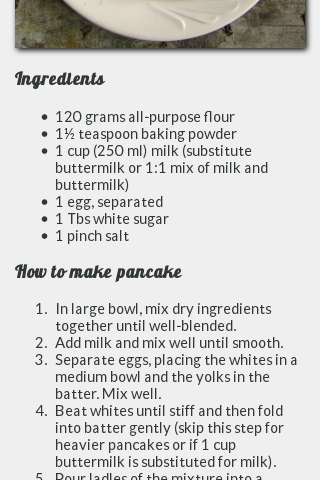
\includegraphics[scale=0.4]{pancakelow2.png}
    \caption{Recipe overview in a low resolution}
    \label{fig:pancakelow}
  \end{center}
\end{figure}

After having developed the calendar, it made sense to work on the recipes. The recipes are the core element of the site and also the most tricky to accomplish.
The issues when developing the recipe pages was mostly aesthetics as there is a need for the website to not feel uninviting to a mobile user and still re-flow good enough to feel inviting for the standard resolution user. Once again, this is pretty much about vertical or horizontal placement of the content. Part of this difference can be seen by comparing figures \ref{fig:pancakelow} and \ref{fig:pancakestd}.

The recipe page can be divided into logical units consisting of the following:

\begin{enumerate}
\item Title
\item Food picture
\item Declaration of content (ingredients and such)
\item The actual recipe
\item Nutrition values
\item Servings information
\item Commentary
\end{enumerate}

\begin{figure}[!h]
  \begin{center}
    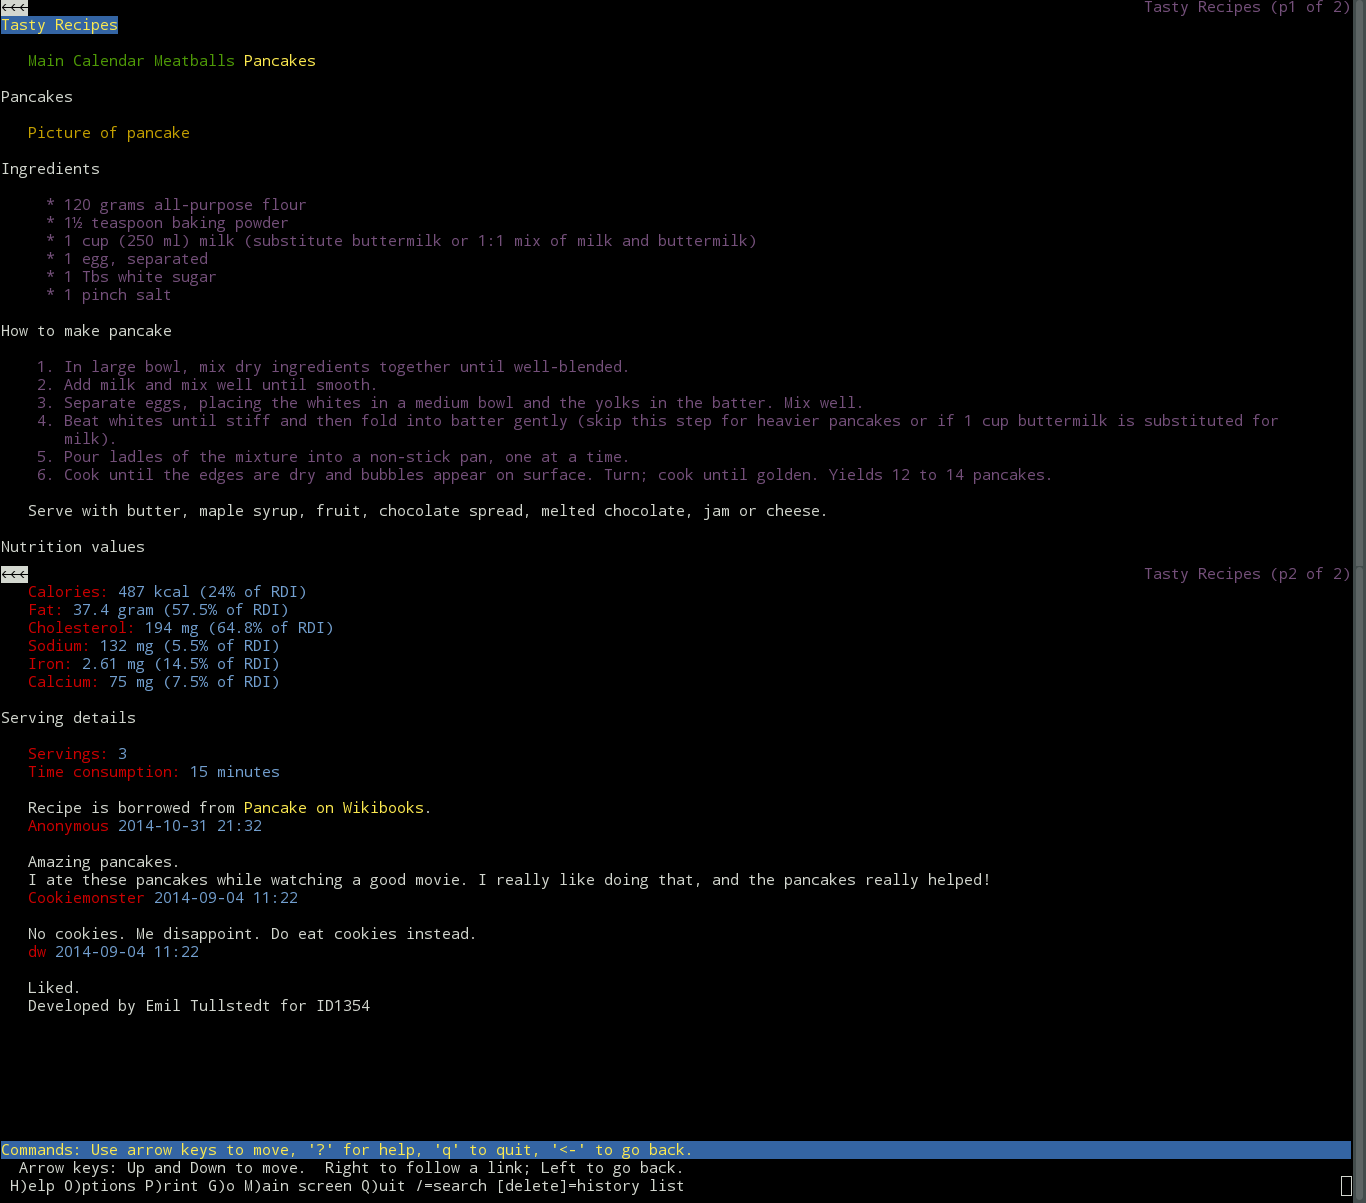
\includegraphics[scale=0.3]{pancakelynxboth.png}
    \caption{The recipe page in a text based browser}
    \label{fig:pancakelynx}
  \end{center}
\end{figure}

\begin{figure}[!h]
  \begin{center}
    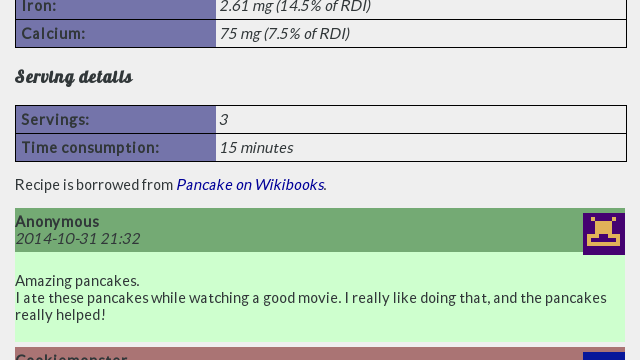
\includegraphics[scale=0.3]{pancakemedium1.png}
    \caption{The pancake recipe as shown on in the mediumlow resolution}
    \label{fig:pancakemedium}
  \end{center}
\end{figure}

\begin{figure}[!h]
  \begin{center}
    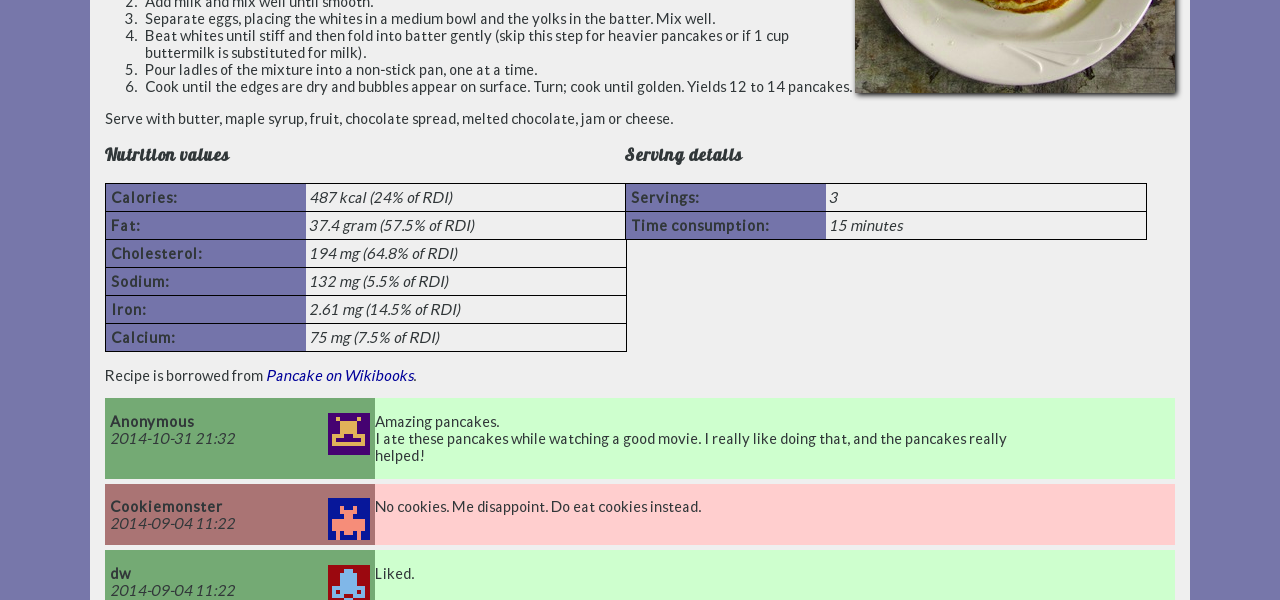
\includegraphics[scale=0.3]{pancakehigh1.png}
    \caption{The pancake recipe as shown on in high resolution - note how the significant difference between this and figure \ref{fig:pancakestd} is that the high resolution version places nutrition values and servings recommendations side-by-side to save vertical space.}
    \label{fig:pancakehigh}
  \end{center}
\end{figure}

Once again, it makes a whole lot sense to look at the website without CSS as in figure \ref{fig:pancakelynx} to ensure this layout is logical even for people who haven't got access to a modern browser. When having made sure the layout makes sense in the terms of HTML, it's not a difficult task to make the CSS that accompanies the site for the different sizes.

There really isn't many newly introduced techniques in the recipe page, mostly reusing what was used to make the calendar in a clever way. Unfortunately, as CSS isn't a programming language, code reuse generally doesn't mean you don't have to write the code again, but the techniques are shared between the calendar and the recipe site.

One difference that can be noted between the high and mediumlow resolutions figures \ref{fig:pancakehigh} and \ref{fig:pancakemedium} is how the comments are re-flowed to save horizontal space by having their user information above the comment rather than to the left of it in the lower resolutions, while in standard resolution and above the vertical space is more interesting and thus the user information is placed left to the comment. By using \texttt{media queries}, this was quite easily accomplished.

When having done the pancake recipe, it was just a matter of entering different data for the meatballs recipe. The difference between these two pages are simply a matter of content.

\subsection{index.html}
\lstinputlisting[language=HTML]{../p1/index.html}

\subsection{calendar.html}
\lstinputlisting[language=HTML]{../p1/calendar.html}

\subsection{meatballs.html}
\lstinputlisting[language=HTML]{../p1/meatballs.html}

\subsection{pancakes.html}
\lstinputlisting[language=HTML]{../p1/meatballs.html}

\subsection{main.css}
\lstinputlisting[language=HTML]{../p1/css/main.css}

\section{Discussion}

\subsection{Basic Requirements}
\begin{itemize}
\item \textbf{Install a web server} - See subsection \ref{subsec:httpd} for details.
\item \textbf{Create HTML and CSS files} - As per section \ref{sec:results} the code validates as shown in figure \ref{fig:valid}.
\item \textbf{Following basic heuristics for user interface design} - this is implied by section \ref{sec:results}.
\end{itemize}

\begin{figure}[!h]
  \begin{center}
    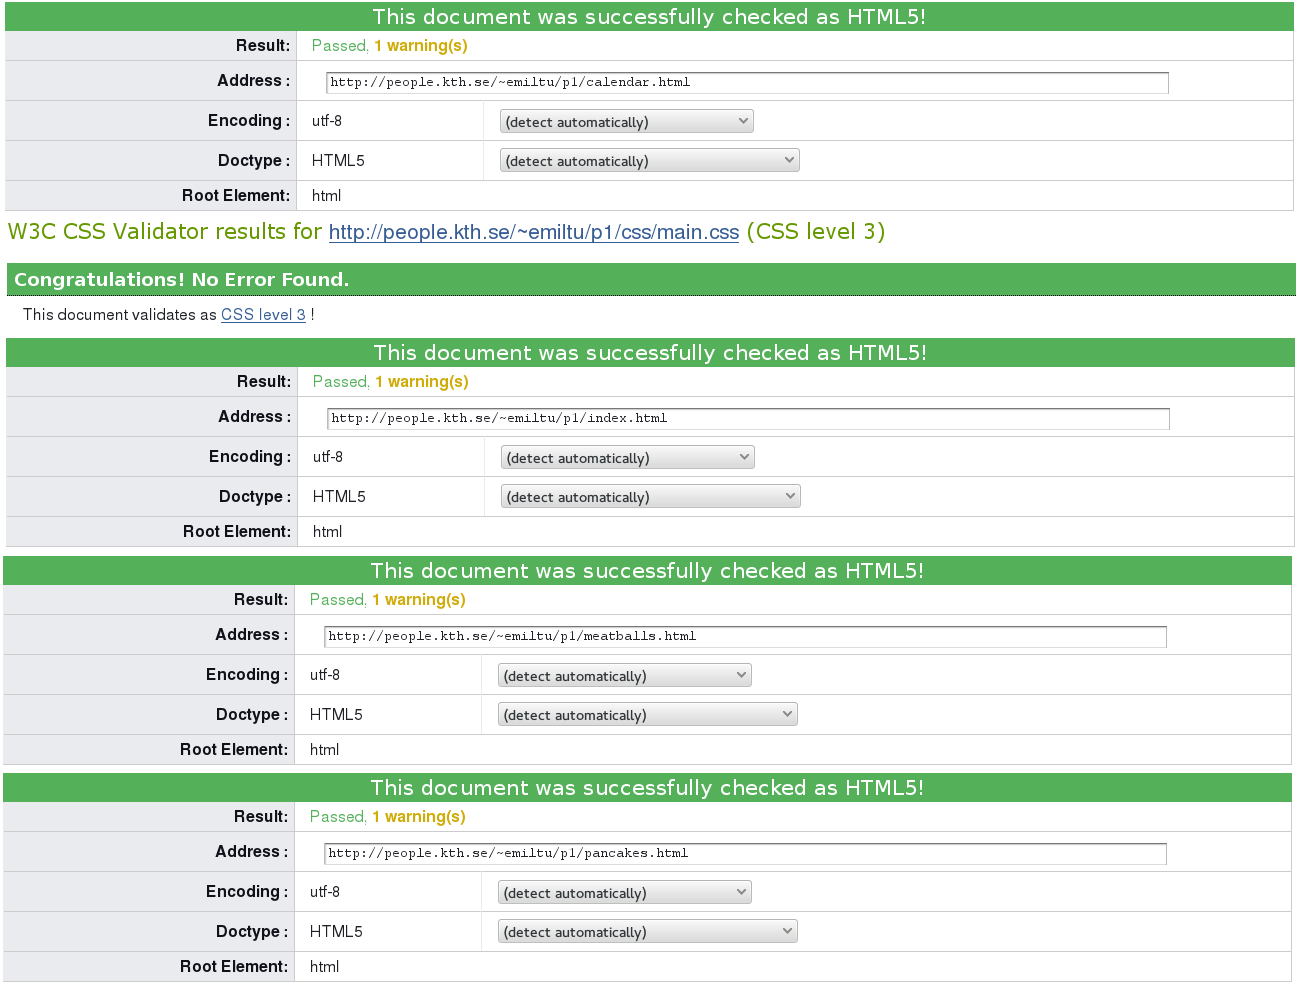
\includegraphics[scale=0.3]{valid.png}
    \caption{Validation results for the different parts of the site}
    \label{fig:valid}
  \end{center}
\end{figure}

\subsection{Adaptiveness}

\begin{figure}[!h]
  \begin{center}
    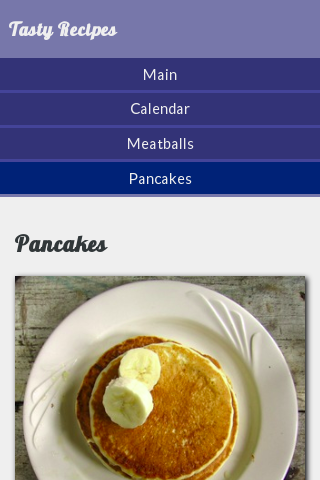
\includegraphics[scale=0.3]{pancakelow1.png}
    \caption{How the menu adapts for lower resolutions}
    \label{fig:menu-adapt}
  \end{center}
\end{figure}

The site is built to feel responsive and work under any browser. By using the built-in Firefox "responsive web development" toolkit this was able to be tested for every change of the page. With the utilization of media queries, the site makes sense on all kinds of different sized screens.

\subsection{Cross-Browser Compatibility}

The site was developed with using "safe" standards in mind, which means that the website \textit{should} work under any modern browser. This was further tested using Microsoft's screenshot service to take screenshots in all different kinds of browsers\footnote{This can be done by the reader by pointing the tool at http://modern.ie/screenshots to the website at http://people.kth.se/$\sim$emiltu/p1}.

\subsection{Web Server Information}
\label{subsec:httpd}

Setting up a web server on Fedora is a matter of \texttt{yum install httpd} and \textit{systemctl start httpd}. This server can then be extended to accommodate server side page generation, such as PHP or WSGI for Python, which is yet to be done.

\begin{lstlisting}
unary Projects/id1354 $ yum info httpd                                                                                                       
Loaded plugins: langpacks

Installed Packages
Name        : httpd
Arch        : x86_64
Version     : 2.4.10
Release     : 1.fc20
Size        : 3.8 M
Repo        : installed
Summary     : Apache HTTP Server
URL         : http://httpd.apache.org/
License     : ASL 2.0
Description : The Apache HTTP Server is a powerful, efficient, and extensible
            : web server.
\end{lstlisting}

\end{document}
